%! Author = adnansiddiquei
%! Date = 13/12/2023

\subsection{Dataset A}\label{subsec:dataset-a}
\subsubsection{Question 1a}\label{subsubsec:q1a}
    \begin{figure}[htb]
    \centering
    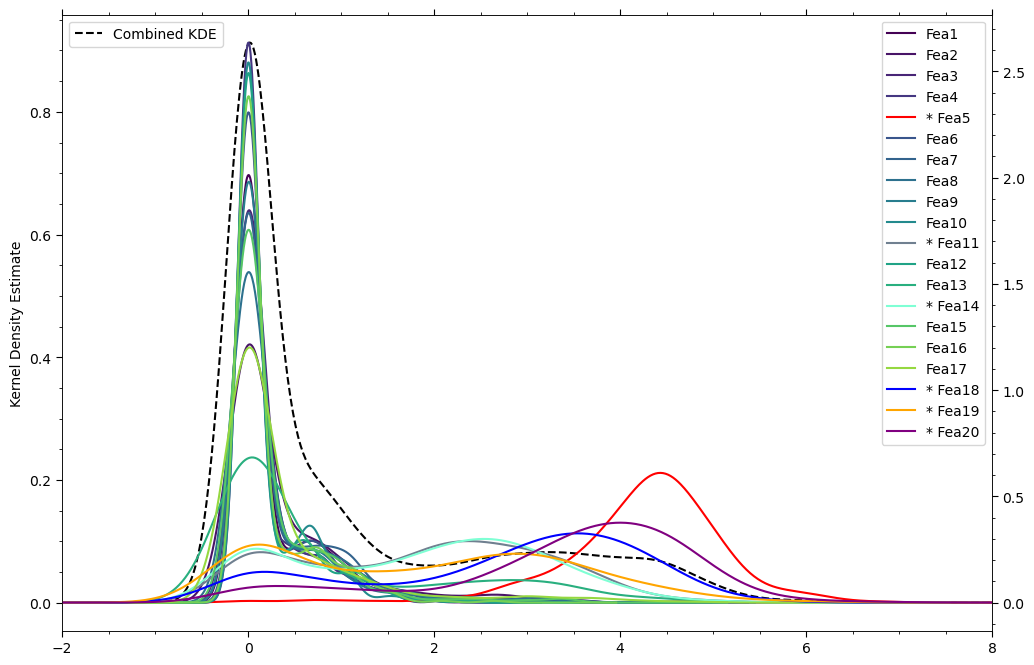
\includegraphics[width=0.9\textwidth]{./figures/q1a}
    \caption{A kernel density estimate of the first 20 features of the \inlinecode{A_NoiseAdded.csv} dataset, which has 20
    plots in total, with the legend and corresponding y-axis on the right. A combined KDE has also been plotted, with
    it's corresponding x-axis on the left. 7 of the 20 features have been highlighted in the legend with an asterisk,
    and have been coloured in slightly more contrasting colours and plotted with a dotted line. These features have a
    larger variance in their density, and are therefore more likely to be more discriminative.}
    \label{fig:q1a}
    \end{figure}

    Fig\eqref{fig:q1a} shows the combined and separated kernal density estimates of the first 20 features of the dataset.
    Several conclusions can be drawn from this plot.
    For most of the features, the KDE is concentrated around the zero value with very little variance, with the exception
    of 7 features: 5, 11, 13, 14, 18, 19 and 20.
    These features are likely to be more discriminative within classification algorithms, as they contain more variability.

\subsubsection{Question 1b}\label{subsubsec:q1b}

    \begin{figure}[htb]
    \centering
    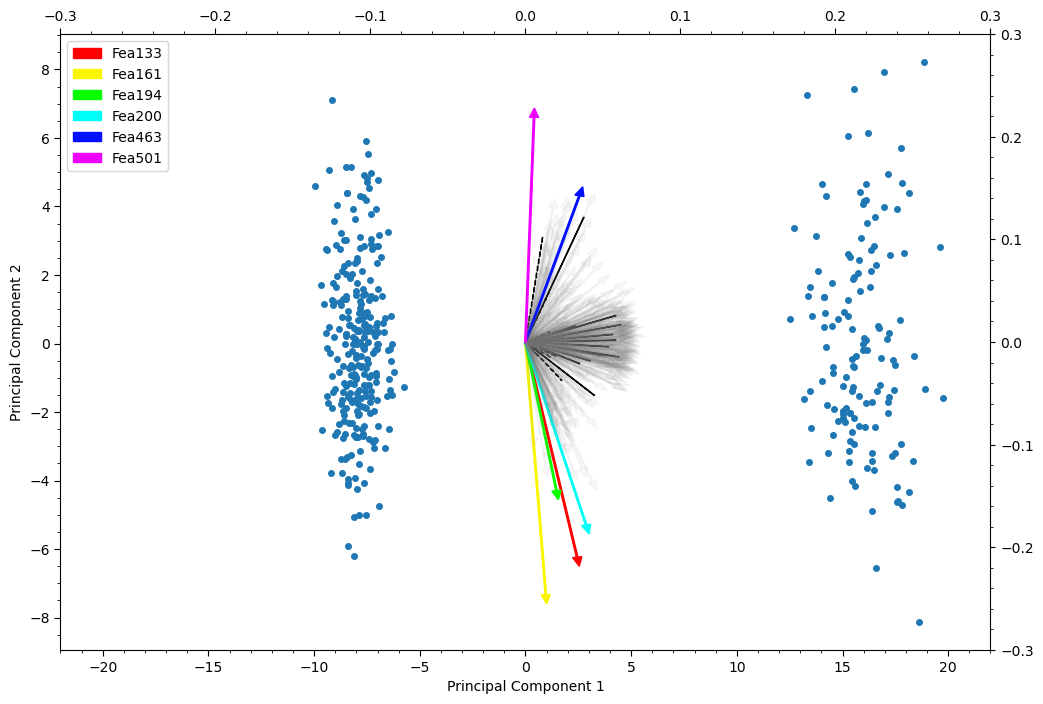
\includegraphics[width=0.9\textwidth]{./figures/q1b}
    \caption{A biplot of the first two principal components in the dataset.
        The coloured arrows indicate the first two principal component loading vectors for every feature which contributes to
        either principal component more than 2\%, these are the most discriminative features.
        Every other loading vector has been plotted in very light grey so their general directions and magnitudes are
        visible.
        The loading vectors for the first 20 features have also been plotted in darker black lines, with the dotted
        black lines corresponding to the dotted KDEs in Fig\eqref{fig:q1a}.
        The loading vectors use the right and top axis of the plot.
        The blue dots indicate the scores for each observation in the dataset for the first two principal components.
        The scores use the left and bottom axis of the plot.
        All four axis are symmetric about the origin for ease of comparison.}
    \label{fig:q1b}
    \end{figure}

    The biplot in Fig\eqref{fig:q1b} shows a PCA of the entire dataset, after standardisation has been applied to each
    feature.
    The coloured arrows indicate the loadings of the features which contribute more than 2\% to either principal
    component, which implies that none of the first 20 features are particularly discriminative.
    An interesting observation is that the most discriminative features are very disciminative with respect to the
    second principal component, whereas the less discriminative features (of which there are many, many more of) are
    more discriminative with respect to the first principal component.
    As a result, the scores on the biplot for the observations w.r.t. the first two principal components separate the
    observations more along the first principal component, rather than the second.
